\section{Copper --- Fermi surface}
\label{sec6:copper}

\begin{itemize}
\item Outline: {\it Obtain MLWFs to describe the states around the Fermi-level in copper.}
\end{itemize}

\begin{figure}[h!]
\centering
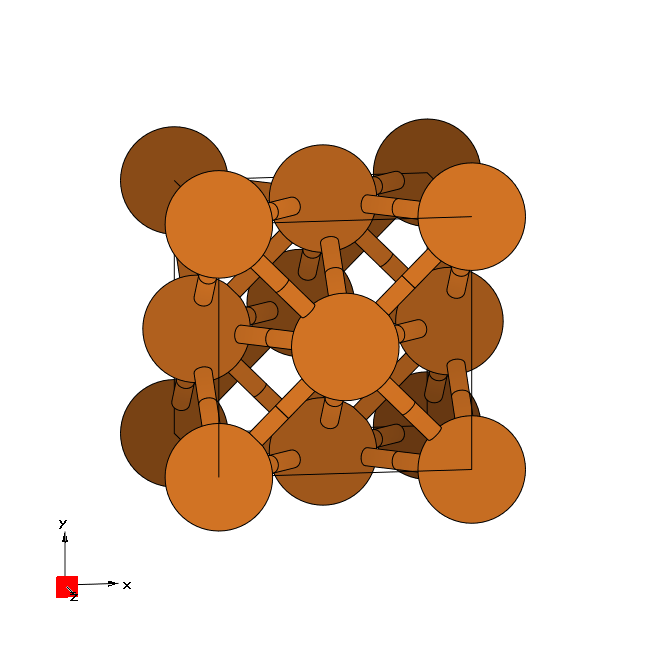
\includegraphics[width=0.25\columnwidth,trim={45pt 45pt 55pt 55pt},clip]{figure/example04/copper_crystal.png}
\caption{Unit cell of Copper crystal plotted with the \xcrysden{} program.}
\label{fig6.0}
\end{figure}

After checking that the calculations have converged as shown in Example \ref{sec5:diamond}, one can proceed with other points in the example.
\begin{enumerate}
	\item {\it Use Wannier interpolation to obtain the Fermi surface of copper.}

	To obtain the value of the Fermi energy we can use the {\tt grep} command (only for Linux/Unix systems) as:
	{\tt\begin{quote}
	\$ > grep Fermi nscf.out
	\end{quote}
    }
	The output should be:
	{\tt
    \begin{quote}
	     the Fermi energy is    12.9344 ev
	\end{quote}
    }
	Alternatively, one can open the {\tt nscf.out} file with the editor of choice and search for "Fermi" inside the file. 
	We can then use this value in the {\tt .win} file to compute the Fermi surface as done in Example \ref{sec2:lead}.
	The interpolated Fermi surface is shown in \Fig{fig6.1}-(a).
	\begin{figure}[h!]
	\centering
	\subfloat[]{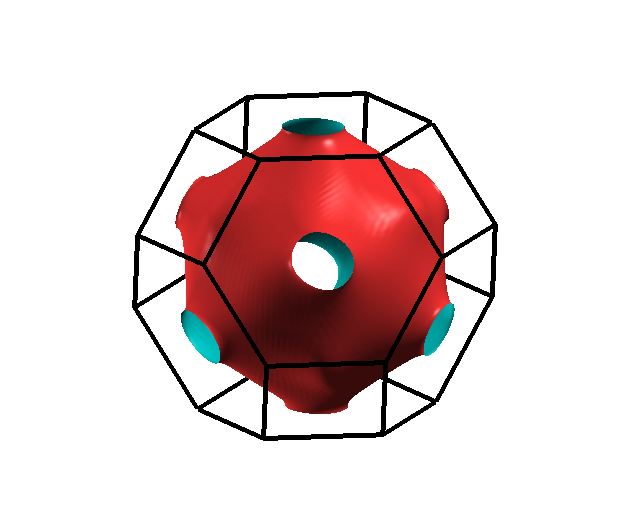
\includegraphics[width=0.3\columnwidth]{figure/example06/copper_fermi_surface.png}}
	\centering
	\subfloat[]{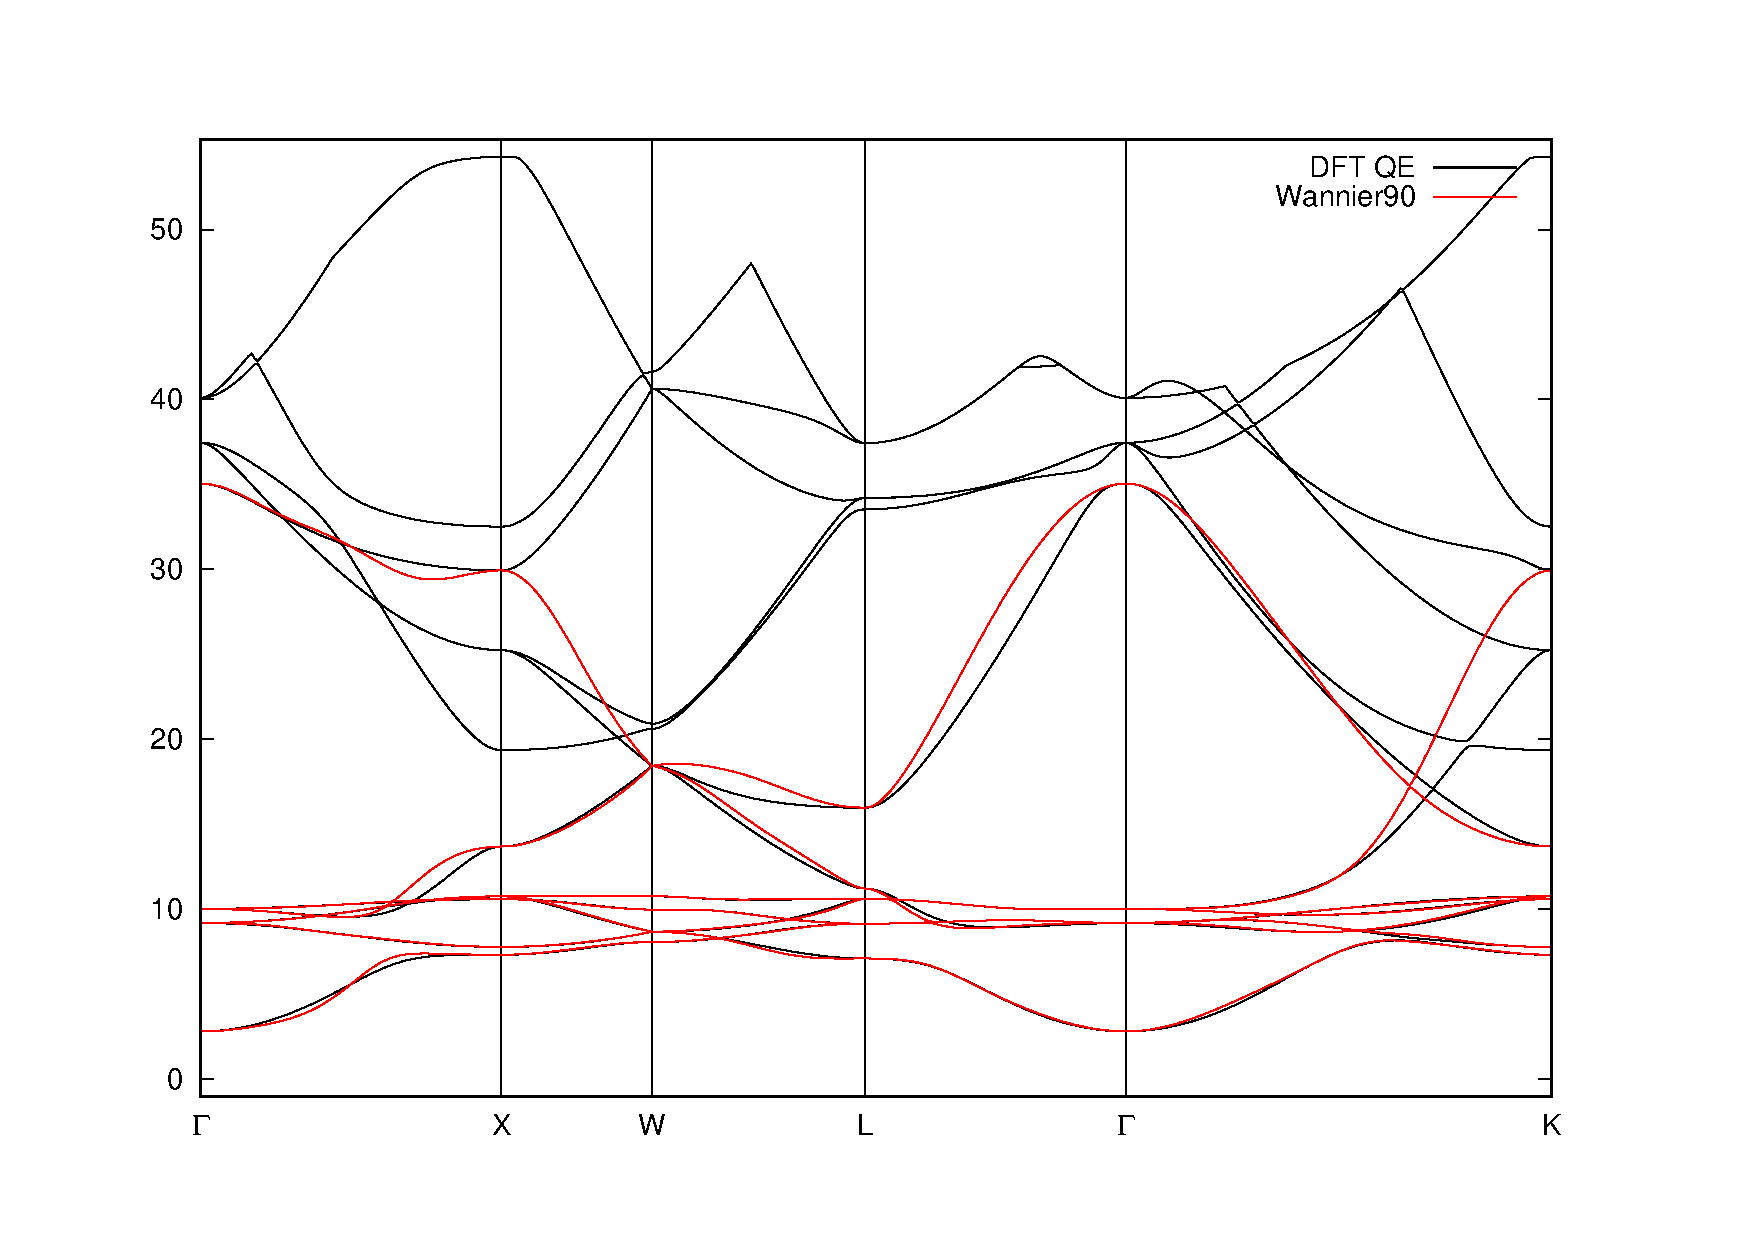
\includegraphics[width=0.7\columnwidth]{figure/example06/copper_DFT_vs_W90_band_structure.pdf}}
	\caption{a) Fermi surface of Copper. b) Band structure of Copper along the $\Gamma$--X--W--L--$\Gamma$--K computed from a non-scf DFT calculation (solid black) and via Wannier interpolation (solid red).}\label{fig6.1}
	\end{figure}
	\item {\it Plot the interpolated bandstructure.}
	
	Bandstructure is shown in \Fig{fig6.1}-(b). One way to obtain the DFT bandstructure on exactly the same path as the one in the {\tt .win} input file, is given by the {\tt bands.x} program available at \url{http://www.tcm.phy.cam.ac.uk/~jry20/bands.html}.
\end{enumerate}
\begin{figure}[h!]
\centering
\subfloat[]{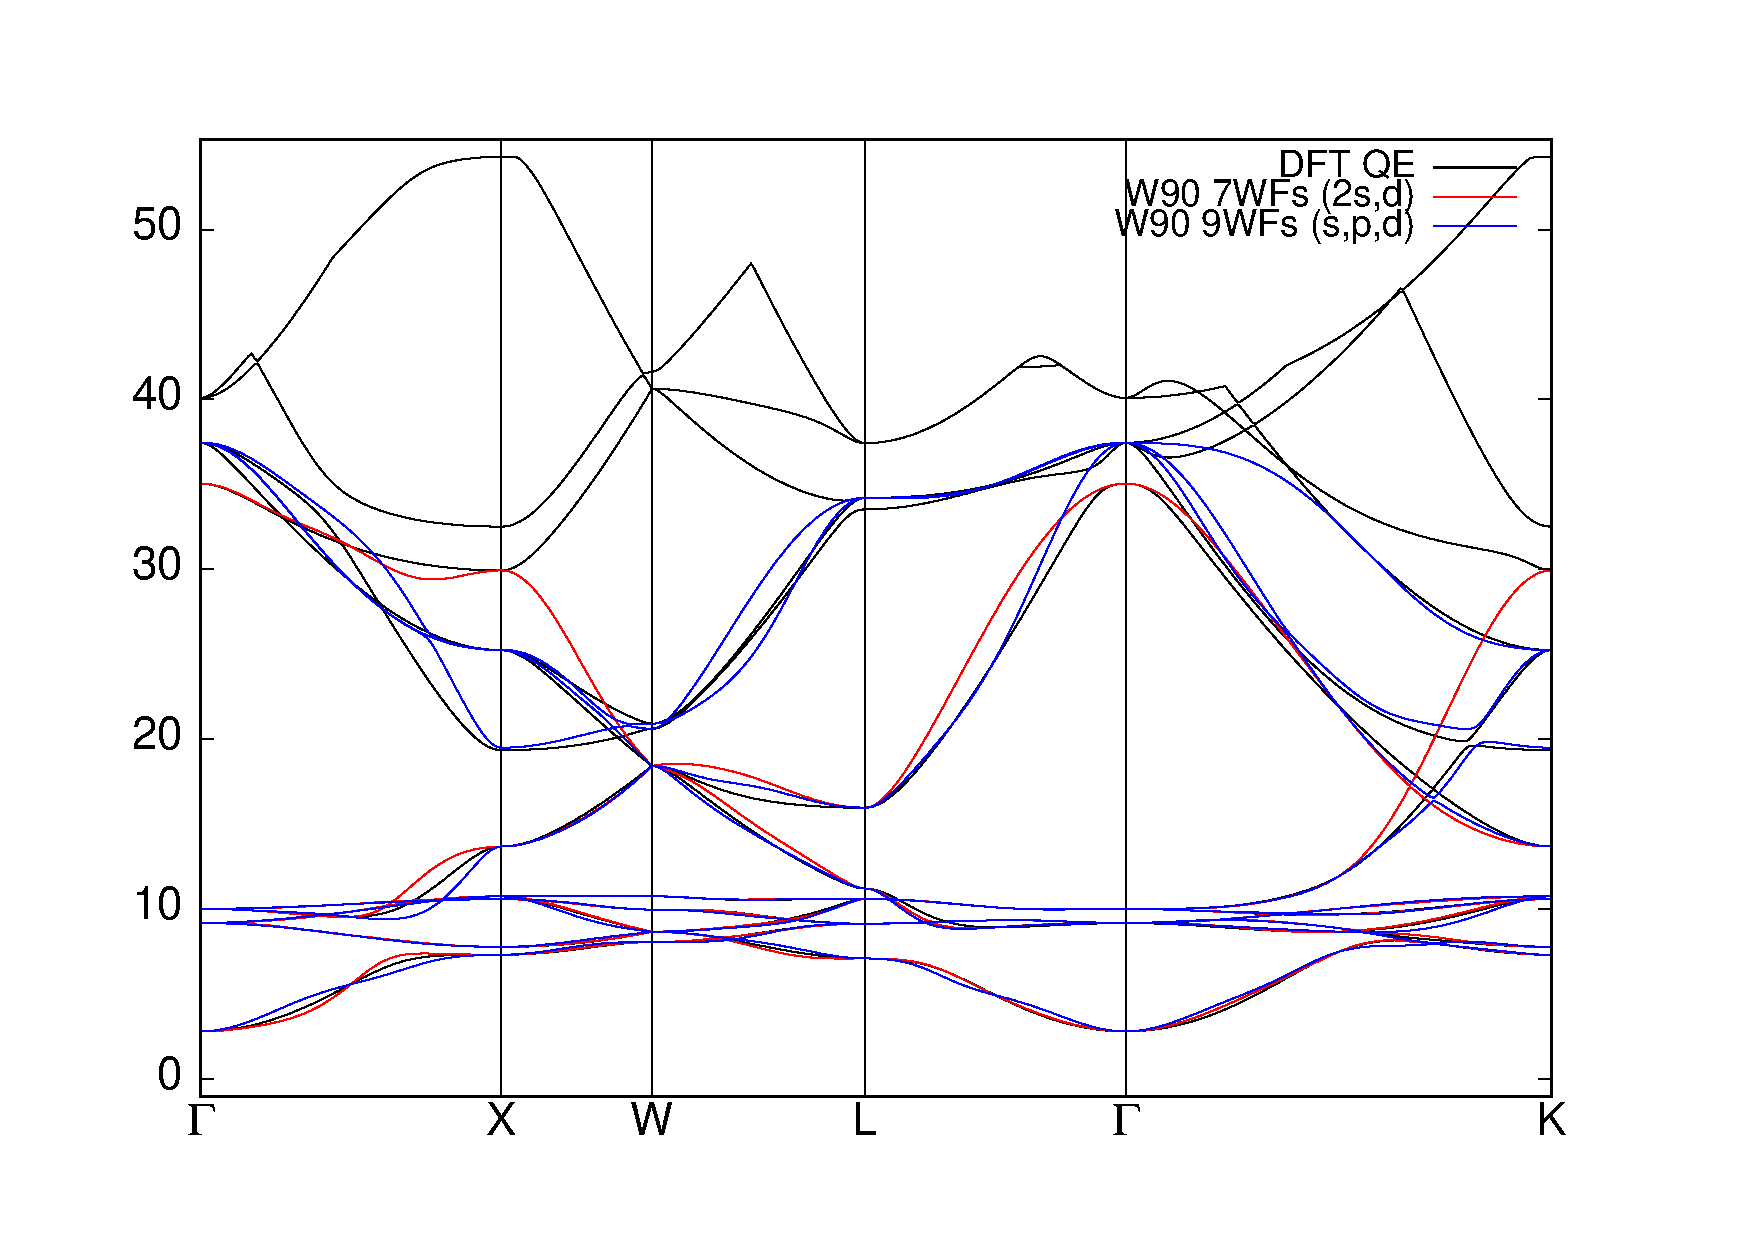
\includegraphics[width=0.45\columnwidth,trim={20pt 20pt 20pt 20pt},clip]{figure/example06/copper_DFT_vs_W90_different_WFs.pdf}}
\subfloat[]{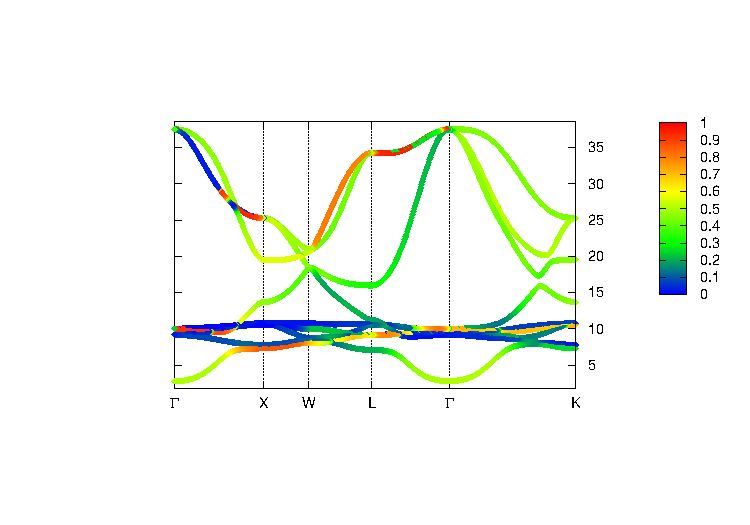
\includegraphics[width=0.60\columnwidth,trim={20pt 40pt 0pt 20pt},clip]{figure/example06/copper_spd_projections_pcolored.pdf}}
\caption{a) Bandstructure of Copper along the $\Gamma$--X--W--L--$\Gamma$--K from a non-scf DFT calculation (solid black) and via Wannier interpolation using two different sets of initial projections, namely $2s$ and 5$d$ ($N_w =7$) (solid red) and 1$s$ 3$p$ and 5$d$ ($N_w=9$) (solid blue). b) $p$ character of bands computed using {\tt bands\_plot\_project = 2,3,4} in the input file. A color scheme is used to measure the $p$ {\it character} of the bands.}\label{fig6.2}
\end{figure}

\begin{tcolorbox}[colback=blue!5!white,title=BANDS.X MINITUTORIAL,float]
    {\small 
    Here we summarize the main steps to produce the bandstructure with the {\tt bands.x} code:

	\begin{itemize}
	\item Compilation: {\tt \begin{quote}
     eg. g95 -o bands.x bands.F90

         ifort -o bands.x bands.F90

    
    for NAG
     
         f95 -o bands.x bands.F90 -DNAG
         \end{quote}

    }

    \item Usage: First you need to generate an {\tt copper.inp} file, with the following structure
  
    \begin{verbatim}
    ! Input file for Copper
    !
    ! First the unit cell (in atomic units = Bohr)
    -3.411 0.000 3.411
     0.000 3.411 3.411
    -3.411 3.411 0.000
    
    !then the number of points along the 1st special path
    100

    ! then the special kpoints and their labels
    G 0.00  0.00  0.00    X 0.50  0.50  0.00
    X 0.50  0.50  0.00    W 0.50  0.75  0.25
    W 0.50  0.75  0.25    L 0.00  0.50  0.00
    L 0.00  0.50  0.00    G 0.00  0.00  0.00
    G 0.00  0.00  0.00    K 0.00  0.50 -0.50
    \end{verbatim}

    Then you need to generate the kpoint list by running the {\tt bands.x} program with the {\tt -pp} flag
    {\tt
    \begin{quote}
     \$ > ./bands.x -pp copper
    \end{quote}
    }
    This will read data from {\tt copper.inp} and write kpoints into {\tt copper\_band.kpt}. 

    {\bf WARNING}: if you already have a {\tt copper\_band.kpt} file from a previous Wannier90 calculation, running the above command will overwrite it.

    Now you need to calculate a non-scf or bands calculation with Quantum ESPRESSO on the k-points given in {\tt copper\_band.kpt}. To do so, copy the {\tt copper.nscf} to {\tt copper.bands} and modify it accordingly. Run a non-scf calculation
    {\tt
    \begin{quote}
    \$ > pw.x < copper.bands > copper.pwscf
    \end{quote} 
    }
    {\bf WARNING}: the output file must terminate with {\tt .pwscf} in order to be read by {\tt bands.x}.

    Now extract the bands from the {\tt copper.pwscf} file 
    {\tt
    \begin{quote}
    \$ > bands.x copper
    \end{quote}
    }
    The bands are written into {\tt copper\_band.dat}. WARNING: if you already have a {\tt coppper\_band.dat} file and a {\tt copper\_band.gnu} file from a previous Wannier90 calculation, running the above command will overwrite them.

    Plot with gnuplot
    {\tt
    \begin{quote}
    \$ > gnuplot --persist copper\_band.gnu
    \end{quote}
    }
\end{itemize}
}
    \end{tcolorbox} 

\begin{enumerate}
	\item [Extra 1:] {\it Compare the Wannier interpolated bandstructure with the full pwscf bandstructure. Obtain MLWFs using a denser k-point grid.}

    

    \item [Extra 2:] {\it Investigate the effects of the outer and inner energy windows on the interpolated bands.} 

    The effect of different energy windows has already been discussed in the Example \ref{sec4:copper}, so it won't be repeated here.

    \item [Extra 2:] {\it Instead of extracting a subspace of seven states, we could extract a nine dimensional space (i.e., with $s$, $p$ and $d$ character). Examine this case and compare the interpolated bandstructures.}

    Using $s,p$, and $d$ orbitals as initial guesses for the \MLWFs{} of Copper, yields the bandstructure (solid blue) shown in \Fig{fig6.2} (with reference values for the inner and outer windows). The bandstructure obtained starting from $2s$ and $5d$ orbitals is shown in red, whereas the DFT reference bandstructure, computed with the procedure described above, is in black. It is clear from \Fig{fig6.2}(a), and \Fig{fig6.2}(b) that the bands of interest have very little $p$ character, particularly the 5 flat bands, which are well very described by $d$ states. 

\end{enumerate}
